\documentclass[a4paper, 12pt]{article}
\usepackage[top=2cm, bottom=2cm, left=2cm, right=2cm]{geometry}
\usepackage[utf8]{inputenc} 
\usepackage{amsmath}
\usepackage{amsfonts}
\usepackage{amssymb} 
\usepackage{graphicx} 
\usepackage{float}
\usepackage[brazil]{babel}
\usepackage{indentfirst}
\usepackage{graphicx}
\usepackage{caption}
\usepackage{subcaption}
\usepackage{verbatim}
\usepackage{minted}

\usepackage{hyperref}
\hypersetup{
	colorlinks=true,
	linkcolor=black,
	filecolor=black,      
	urlcolor=blue,
}

\DeclareMathOperator{\sen}{sen}
\renewcommand{\sin}{\sen}
\DeclareMathOperator{\arcsen}{arcsen}
\renewcommand{\arcsin}{\arcsen}
\DeclareMathOperator{\tg}{tg}
\DeclareMathOperator{\arctg}{arctg}
\renewcommand{\arctan}{\arctg}

\title{Projeto de Sistemas Embarcados\\Relatório Final}
\author{Eugênio Piveta Pozzobon\\Mauren Walter D'Avila}
\date{\today}

\begin{document}
	\maketitle
	\newpage
	\tableofcontents
	\newpage
	
	\section{Introdução}
	
	O projeto desenvolvido consiste em um sistema de balança para balanceamento de um veículo (Figura \ref{fig:cornerweithscaleexample}). Esse sistema é amplamente utilizado em equipes de corrida para ajustar a suspensão do veículo para competições, provendo um ajuste fino que pode ser desenvolvido para cada piloto. O Ganho de performance dado por esse ajuste pode fazer a diferença entre vitória e derrota. 
	
	\begin{figure}[!htb]
	\centering
		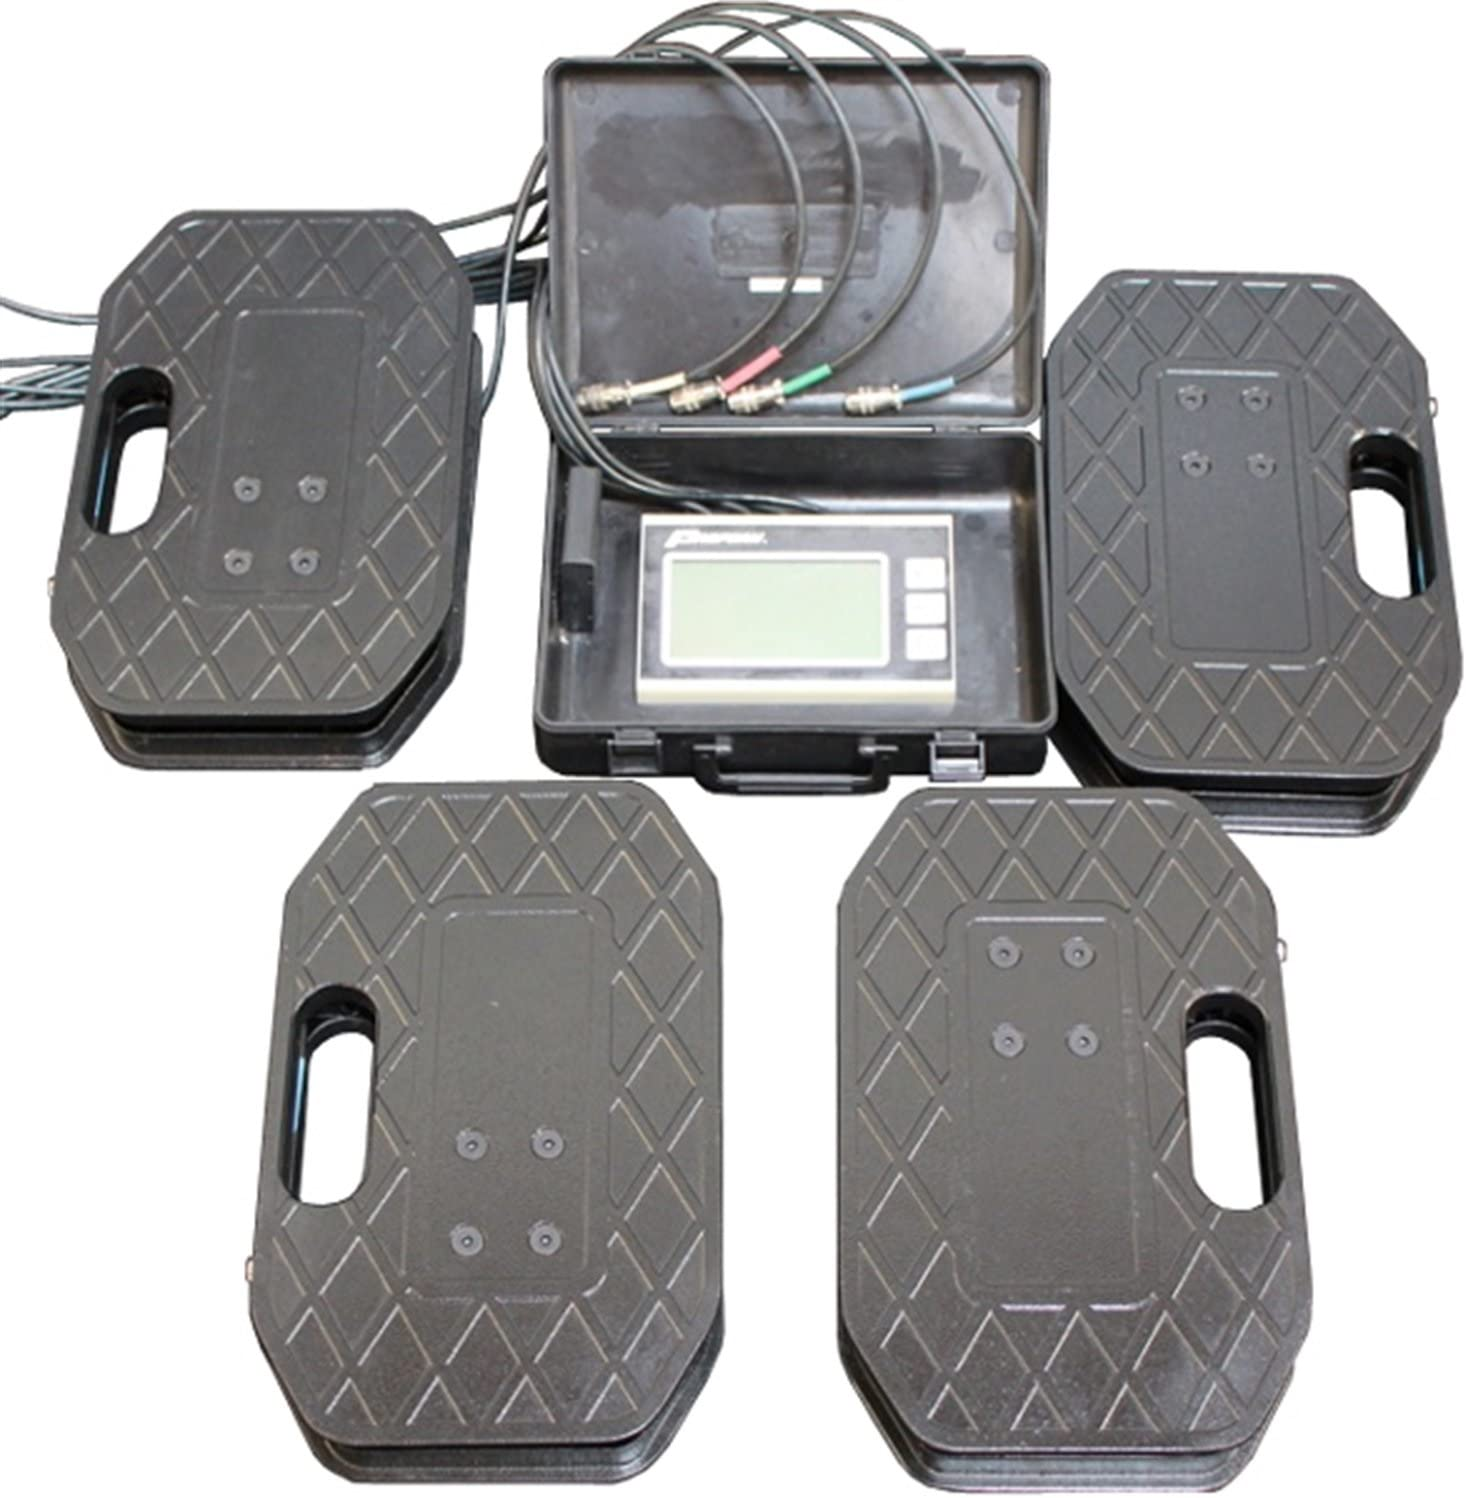
\includegraphics[width=6cm]{
			cornerweithscaleexample}
		\caption{Sistema comercial de Balanças}
		\label{fig:cornerweithscaleexample}
	\end{figure}
	
	A entrada de dados seria feita por um chip HX711, porém preferiu-se realizar uma eletrônica de instrumentação para minimizar o uso de bibliotecas externas e poder dimensionar um sistema adequado para a aplicação. 
	
	Processamento e aramazenamento de dados ocorre pra ler o dado do chip e efetuar a conversão do dado bruto em um peso em uma determinada unidade. Além disso, as balanças precisam ser calibradas com um peso de calibração (5kg) e com isso se obtêm um dado de calibração que é armazenado na \textit{EEPROM} do \textit{ATMEGA328P} para ser utilizado em todas as medições futuras das balanças. 
	
	\subsection{Github}
	O Projeto foi hospedado no Github e pode ser acessado neste link: \url{https://github.com/Eugenio-Pozzobon/Sistema-de-Balancas-Automotivo}
	
	\section{Desenvolvimento Teórico}
	Um sistema que busca realizar a leitura da massa pode usar uma variedade de categorias de sensores, mas a escolhida para este projeto foi uma célula de carga.
	
	\subsection{Célula de Carga}
	
	A célula de carga é um sensor que possibilita aferir a força aplicada sobre um material. É um composto que, quando expandido, aumenta a sua resistência elétrica interna. Essa variação de Resistência pode ser lida por uma Ponte de Wheatstone. A lâmina do sensor pode ser colada em uma peça metálica que estará exposta a tensão e deformação, como a peça da figura \ref{fig:celuladecarga}
	
	\begin{figure}[!htb]
		\centering
		\caption{Célula de Carga}
		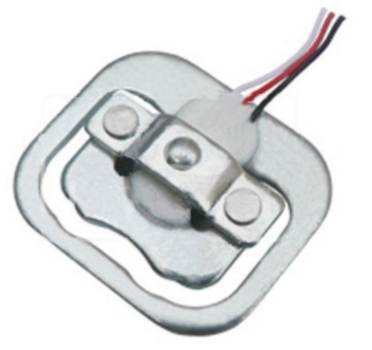
\includegraphics[width=.4\linewidth]{celuladecarga}
		\label{fig:celuladecarga}
	\end{figure}
	
	\section{Ponte de Wheatstone}
	
	A ponte de Wheatstone é uma forma comumente utilizada para medição de variação de resistência. É possível agrupar 4 células de carga que estão montadas em uma balança comercial em uma ponte completa. A ponte completa impede variações de medição em função de situações ambientais como temperatura, e, portanto, é uma ótima forma de aferir a variação da resistência da ponte. 
	
	O circuito da ponte, como demonstrado na figura \ref{fig:circuitoponte}, possibilita que, com uma tensão de excitação de entrada, seja possível obter uma oscilação da tensão de saída, conforme variam-se as resistências. Se as 4 resistências são sensíveis ao peso, então a oscilação do peso afetará a tensão de saída. Essa tensão de saída é dada pela sensibilidade da ponte e a tensão de entrada (excitação) da ponte.
	
	\begin{figure}[!htb]
		\centering
		\caption{Circuito de Operação da Ponte de Wheatstone}
		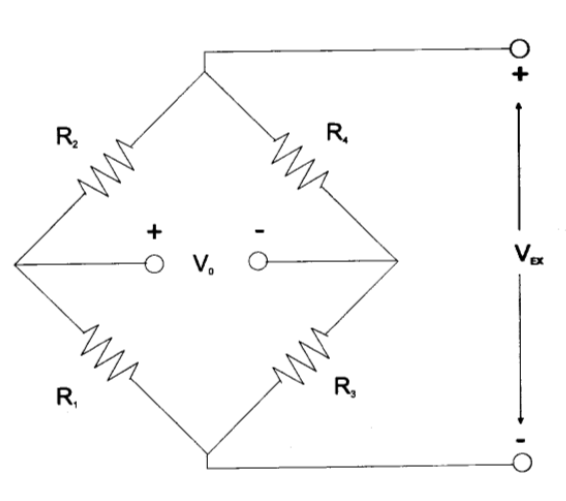
\includegraphics[width=.4\linewidth]{circuitoponte}
		\label{fig:circuitoponte}
	\end{figure}
	
	\subsection{Amplificador de Instrumentação}
	Amplificadores de instrumentação são CIs que amplificam a tensão diferencial de entrada, mantendo alta impedância de entrada, elevada rejeição a sinais de modo comum, e um ganho ajustável por um resistor de ganho.
	
	\subsection{FreeRTOS}
	Foi utilizado o FreeRTOS na criação do sistema embarcado como uma biblioteca de multi-thread (ou multitasking). Esse sistema também é um SO preemptivo, ou seja, permite a execução de tarefas em paralelo de forma que cada tarefa acesse o processador por um certo período de tempo e, ao término, troque automaticamente para a próxima tarefa seguindo a prioridade definida no código. 
	
	\section{Desenvolvimento Prático}
	
\section{Circuito}
O circuito foi desenvolvido usando o Proteus 8.9 para ser simulável em ambiente virtual. Conta com controladores e dispositivos passivos e ativos para montar o sistema de instrumentação embarcado.  

\subsection{ATMEGA328P}
Um controlador de amplo acesso e com ampla documentação disponível é o Atmega 328p que embarca alguns modelos da Série Arduino. Esse controlador possui uma taxa de operação de 8 ou 16MHz que é configurável. Para o projeto, optou-se por simular com 16MHz usando um cristal oscilador acoplado com 2 capacitores de 22pF. Esse controlador também requer um resistor  de \textit{pull-up} na entrada de \textit{Reset}.

Esse controlador possui 6 entradas analógicas em um ADC (Conversor Analógico Digital) que podem ler um sinal com até 10bits de resolução. Considerando que essa unidade consegue ler tensões de 0 a 5V, a resolução de leitura será $ 5\div 1024 = 4,88mV  $

\subsection{Amplificador de Instrumentação}
A leitura dos dados das 4 células de carga que são agrupadas em uma balança comercial como a da Figura \ref{fig:balanca} pode ser feita com uma ponte de Wheatstone. Quando um peso é inserido sobre a balança, isso gera uma oscilação de até $ 1mV $ por $ 1V $ na alimentação. Com uma tensão de excitação da ponte igual a $ 1,3V $ o resultado será uma oscilação de tensão de $ \pm 1,3mV $ que precisa ser amplificado para uma correta leitura para o controlador. 

\begin{figure}[!htb]
	\centering
	\caption{Células de carga distribuídas nas balanças para forma a ponte}
	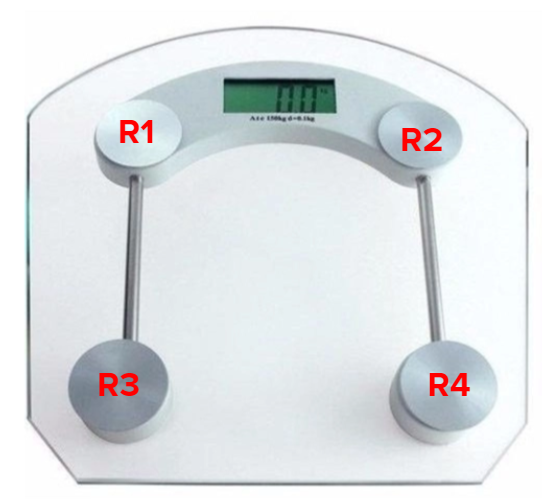
\includegraphics[width=.5\linewidth]{balanca}
	\label{fig:balanca}
\end{figure}

Para isso, foi selecionado o amplificador AD623 (Figura \ref{fig:AD}) que trabalha com uma faixa de ganho de 1 a 1000. A equação \ref{eq:ganho} define o valor de resistor conforme o ganho selecionado. Para uma boa operação, é inserido uma tensão de offset de 2.5V, possibilitando uma leitura negativa da célula, de -100 a 100kg, onde 0kg equivale a 2,5kg. Considerando que o sistema exige uma resolução de 0,5kg, e a resolução mínima de leitura do controlador é $ 5mv $, então, para uma margem de $ \pm100kg $ é preciso uma oscilação na entrada de 1V. Assim, +100kg equivale a 3,5V.

\begin{equation}
	R_G = \dfrac{100k}{(G-1)}
	\label{eq:ganho}
\end{equation}	

\begin{figure}[!htb]
	\centering
	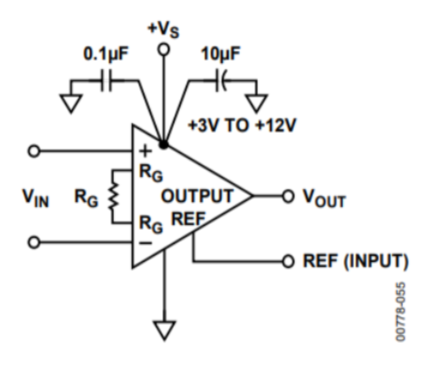
\includegraphics[width=.5\linewidth]{AD623}
	\caption{Diagrama de ligação AD623}
	\label{fig:AD}
\end{figure}

Então, calcula-se que o ganho necessário é de 1V/1,3mV = 770. Dessa forma, pela equação \ref{eq:ganho}, o resistor de ganho do amplificador $ Rg = 130 $. 


\subsection{Outros componentes}

Para o funcionamento do circuito, resta então botões para receber as entradas do usuário, e um LCD que será o display dessas informações. Assim, cria-se o diagrama do sistema (Figura \ref{fig:hardwarefinal}). 

\begin{figure}[!htb]
	\centering
	\caption{Diagrama Final do Circuito}
	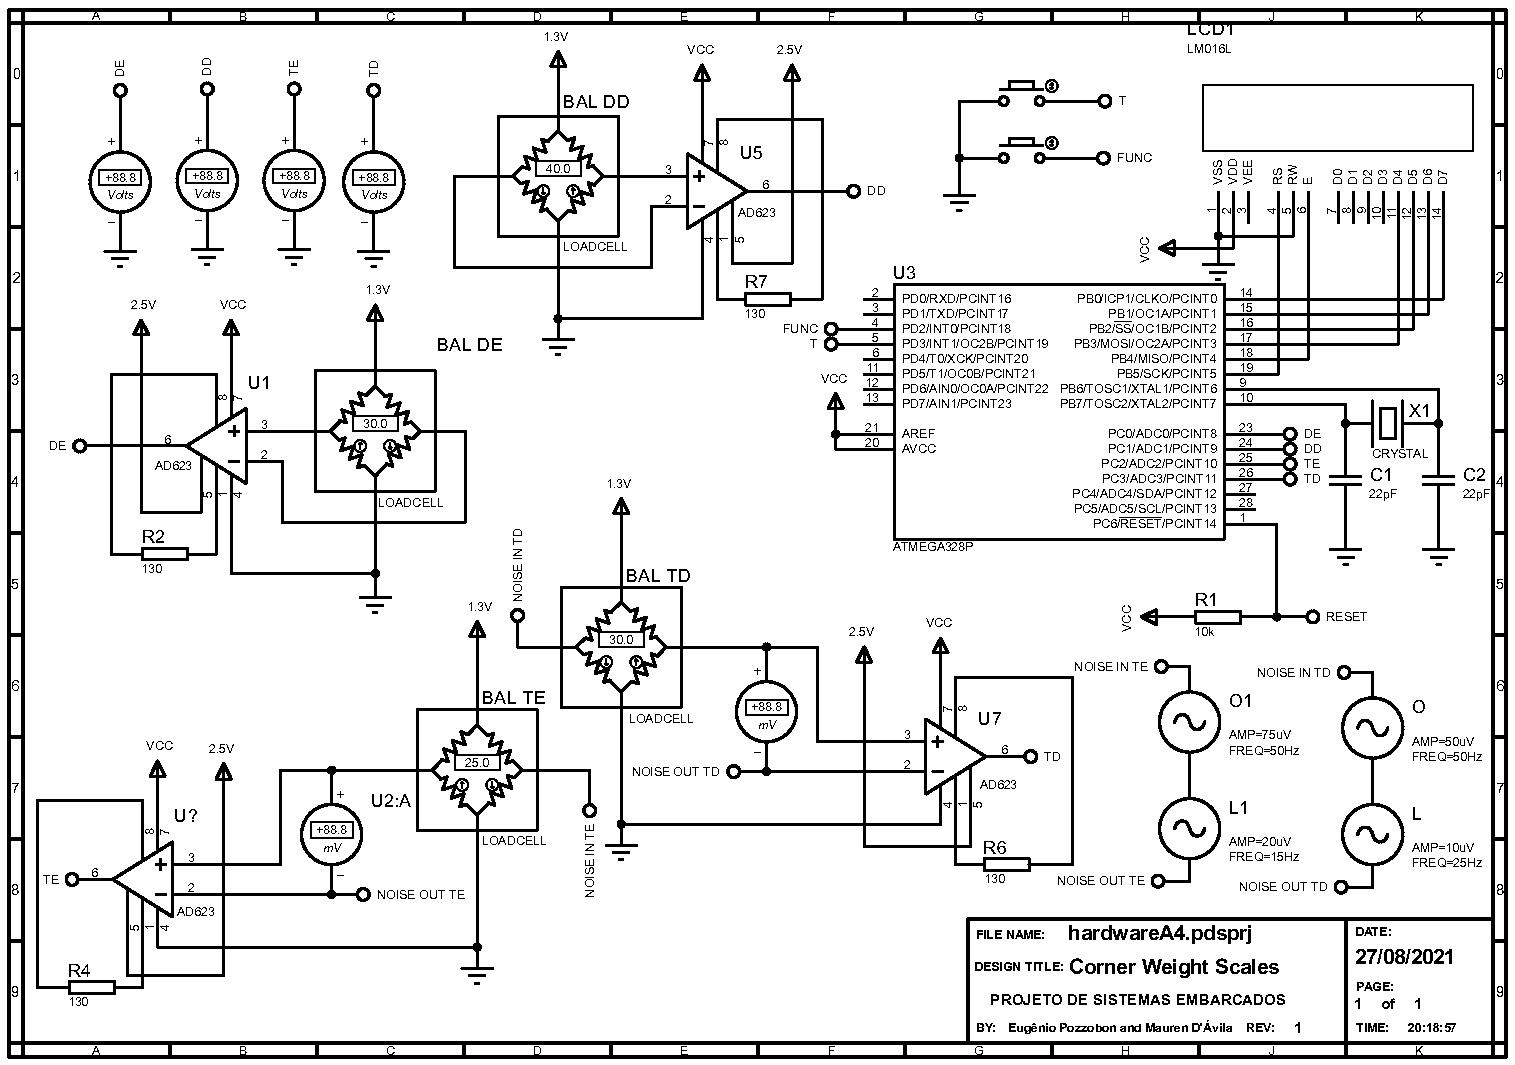
\includegraphics[width=.85\linewidth]{hardwareA4}
	\label{fig:hardwarefinal}
	
\end{figure}

\subsection{Filtragem do sinal}

O Sinal da célula de carga é extremamente sucetível a ruídos. Por isso, é necessário utilizar filtros, sejam eles ativos, passivos, ou digitais. Devido a algumas limitações da simulação, foi possível operacionalizar somente um filtro digital de média móvel.

\subsubsection{Filtro Média Móvel}
O filtro de média móvel é processável digitalmente no controlador. Para isso, é preciso que seja realizado o armazenamento de um buffer de dados, e com esses dados se calculará uma média. Assim, o resultado da média móvel se dá pelo somatório da equação \ref{mediamovel}

\begin{equation}
	R_M = \dfrac{buf_1+buf_2 + buf_3\cdots buf_{n-1} + buf_n}{n}
	\label{mediamovel}
\end{equation}

Como o dado lido no arduino é um valor inteiro com 10 bits, é possível realizar a média móvel, incluindo divisão, com um buffer de tamanho na potência de 2. Assim, é possível operacionalizar a divisão sem ponto flutuante, apenas com bitshift, e poupar processamento do controlador.
O código abaixo demonstra a operacionalização da média móvel.

\begin{minted}{C}
	int32_t mediaMovel(int32_t *array){
		int32_t media = 0;
		for(int i = 0; i<BUFFER_SIZE; i++){
			media += (array[i]);
		}
		return (media >> bitshift);// / BUFFER_SIZE;
	}
\end{minted}

Para cumprir com o objetivo do sistema de obter leituras em $ 0,1kHz $, é preciso averiguar o tempo de processamento. Uma leitura analógica custa $ 100us $ para o ATMEGA, realizar 4 leituras, $ 400us $. Considerando que que $ 0,1kHz = 10ms $, têm-se que o número máximo de leituras em buffer é de $ 10ms\div400us = 25 $. O valor potência de 2 mais próximo é 16 e portanto, esse será o tamanho do buffer lido na média móvel. O tempo extra fica disponível para demais processamentos. 
	
	\subsection{Ambiente de Desenvolvimento}
	
	Foi escolhido utilizar a IDE Clion com Plugin PlatformIO devido a sua integração direta com o Github, possibilitando trabalho em conjunto de forma totalmente remota e compilando diretamente para a raiz de arquivos configurada no Proteus para realizar o upload do código do ATMEGA328P. Por meio desse plugin foi possível configurar um ambiente que rodasse, independente da máquina, tendo acesso as mesmas bibliotecas na raiz de armazenamento da pasta 'lib' e ainda possibilitando a execução de testes unitários com a biblioteca \textit{Unity}. 
	
	\subsection{Tasks FreeRTOS}
	São tarefas assíncronas que rodam com prioridade especificada pelo usuário, essa execução assíncrona é uma característica do sistema operacional, chamada multi-tasking. As tarefas não se executam ao mesmo tempo e o gerenciamento da execução no tempo é tratado pelo scheduler, que decide quando e qual parte do programa deve rodar.
	
	\subsubsection{Leitura de Dados e Processamento}
	Utilizamos para receber os dados das balanças (armazenando no buffer da média móvel) e do estados dos botões. Esse dado posteriormente ainda passava pelos cálculos para transformar o valor lido em um valor em quilograma, aplicando os filtros que foram programados para isso. 
	
	\subsubsection{Atualização do Display}
	
	Devido as diversas operações que o Mecânico precisa realizar no ajuste de suspensão, é preciso que o \textit{display} mostre uma variedade de dados acerca da massa em cada roda, distribuição lateral e longitudinal. Para isso, verificamos o estado atual do botão \textit{'func'} e mediante a isto atualizamos o LCD. (Figura \ref{fig:operacao})
	
	\begin{figure}[!htb]
		\centering
		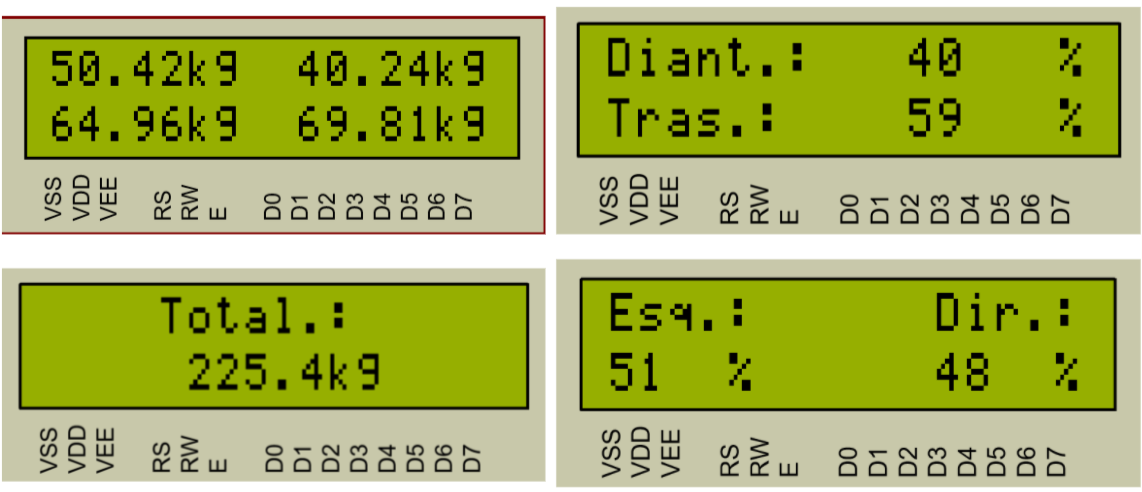
\includegraphics[width=.6\linewidth]{operacao}
		\caption{Simulação das Funções no Display}
		\label{fig:operacao}
	\end{figure}
	
	\subsection{Problemas encontrados}
	\label{poblemas}
	Tivemos algum problema de configuração e operacionalização da IDE escolhida, contudo, após os problemas serem resolvidos, foi muito mais prático de desenvolver o código quando comparamos com o processo da IDE do Arduíno. 

	Além disso, normalmente a leitura e processamento de dados seria a thread mais importante, porém, quando o código é executado com essa ordem de prioridade, a thread para atualização do display nunca é executada. Uma saída encontrada e que funciona adequadamente foi executar um taskDelay na thread de atualização, na taxa de update desejado, e permitir que, durante esse delay, a thread de leitura e processamento seja executada. Dessa forma, não há desperdício de tempo na execução das threads.  
	
	
	\section{Resultados Obtidos}
	Com a correção dos problemas discutidos anteriormente, foi possível simular no Proteus o sistema, inserindo massa nas balanças e verificando os dados do LCD. O filtro digital de média móvel também atendeu as expectativas, pois, com ele, o ruído inserido na simulação não fez com que a massa medida oscilasse além de $ \pm 0,5V $. A figura \ref{fig:simulacao} demonstra a operação da simulação.
	
	\begin{figure}[!htb]
		\centering
		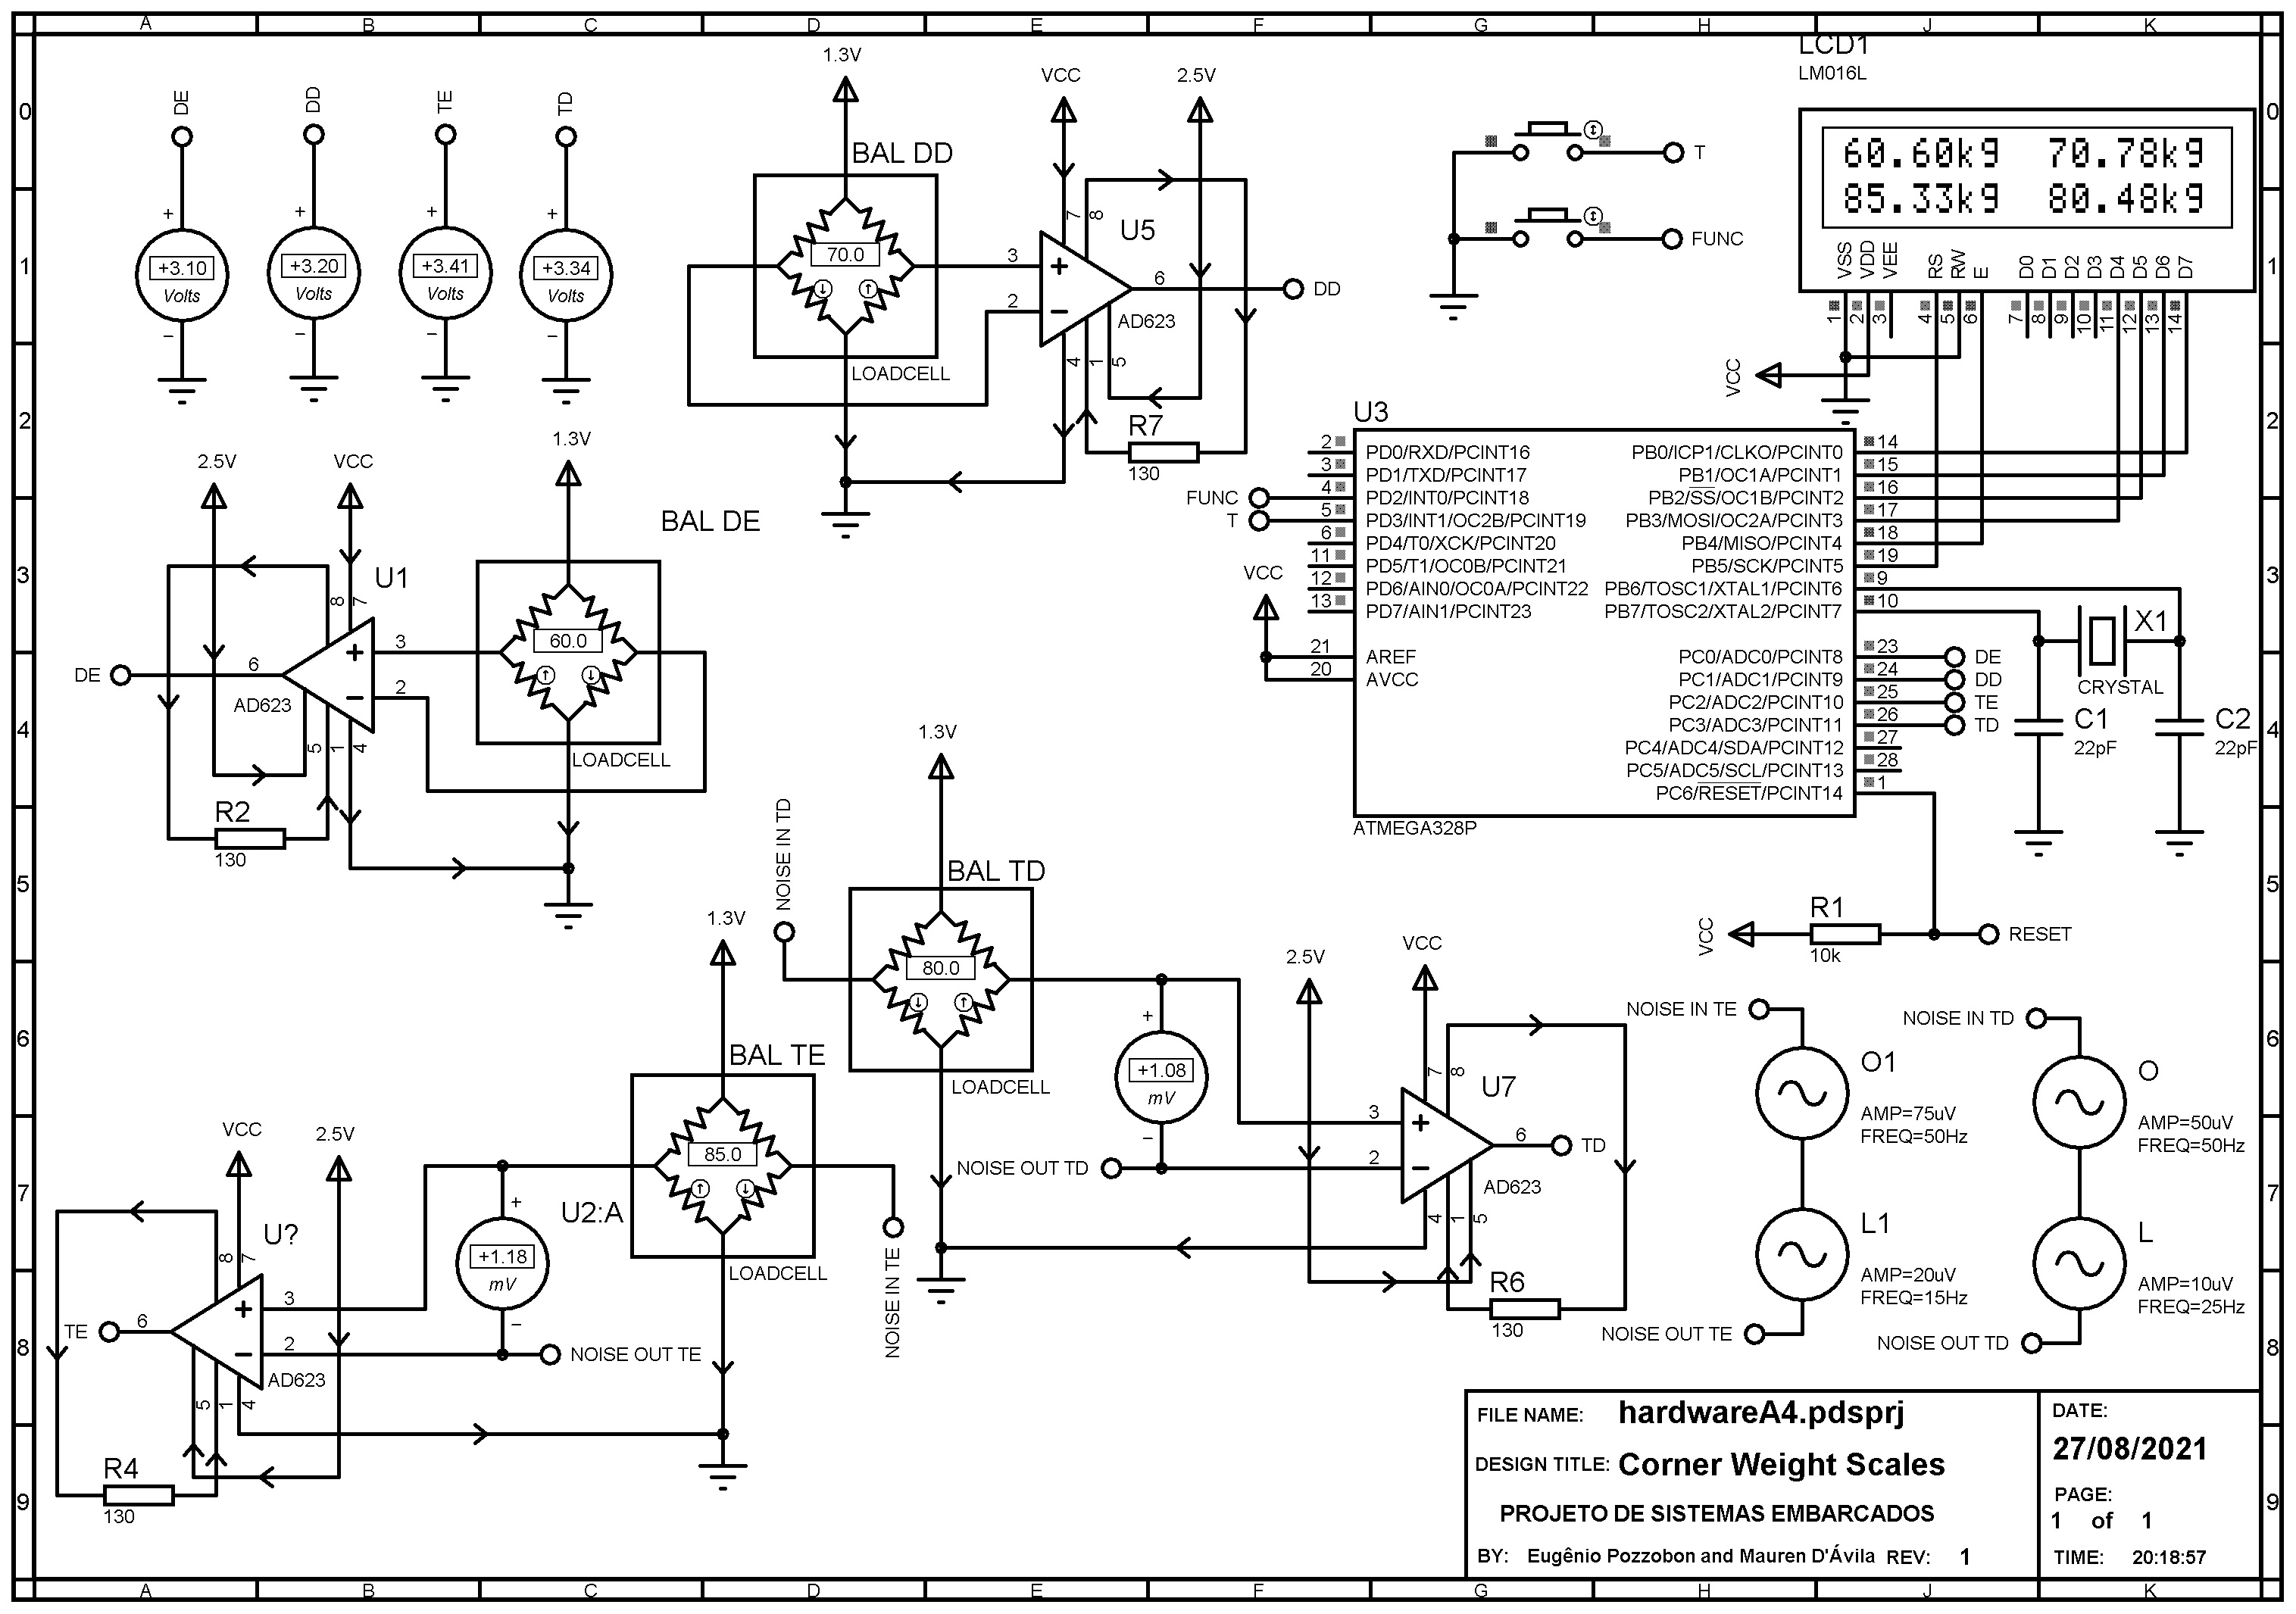
\includegraphics[width=.85\linewidth]{simulacao}
		\caption{Sistema comercial de Balanças}
		\label{fig:simulacao}
	\end{figure}

	Além disso, a tara armazenada na EEPROM permitiu maior dinamicidade nas medições, evitando que uma configuração anterior fosse perdida ao reiniciar o sistema, mesmo na simulação do Proteus.  
	
	\section{Conclusão}
	Foi possível, com esse trabalho, operacionalizar de forma satisfatória o sistema de instrumentação usando um sistema operacional de tempo real. Algumas melhorias de implementação do sistema talvez pudessem abordar a subdivisão das tasks de forma mais profunda, separando leitura do processamento. Contudo, é importante cuidar para que isso não retome o problema discutido na seção \ref{poblemas} e melhore o processamento e armazenamento dos dados de Tara, que também pode ser feito em uma \textit{thread} separada. 
	
	
\end{document}
